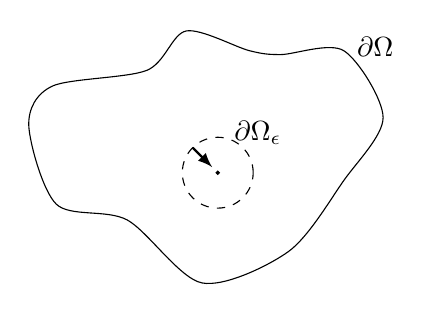
\begin{tikzpicture}
    \begin{scope}[scale = 1]
        \draw plot [smooth cycle] coordinates {(-2, 0) (-1.7, .5) (-.5, .7) (0, 1.2) (.8, .95) (1.2, .9) (2, .95) (2.5, .1) (2, -.7) (1.3, -1.6) (.2, -2) (-.75, -1.2) (-1.65, -1)};
        \draw[dashed] (.4, -.6) circle (.45);
        \draw[fill = black] (.4, -.6) circle (.02) node[below]{$\bzhe$};
        \node at ({.4 + .72*cos(45)}, {-.6 + .72*sin(45)}) {$\partial\Omega_{\epsilon}$};
        \node at (2.4, 1) {$\partial\Omega$};
        \draw[-latex, thick] ({.4 + .45*cos(135)}, {-.6 + .45*sin(135)})--({.4 + .1*cos(135)}, {-.6 + .1*sin(135)});
        \node at ({.4 + .7*cos(135)}, {-.6 + .7*sin(135)}) {$\nhat$};
    \end{scope}
\end{tikzpicture}